\providecommand\docroot{../}
\documentclass[\docroot/main]{subfiles}
\begin{document}
\chapter{Run Baby, Run}
\begin{wrapfigure}{r}{.45\textwidth}\rotatebox{7}{\shadowbox{\begin{minipage}{.45\textwidth}%
  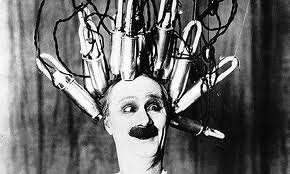
\includegraphics[width=\textwidth]{\docroot/998_figures/mad-science.jpg}
  \caption*{Let's experiment}
\end{minipage}}
}
\end{wrapfigure}
Why not simply run the application?
Give it to willing users and let them do with it, whatever they think it is for?
Call the users beta testers, provide some incentive to report problems, and you are done, right?

Well, for simple applications, like scripts that do just one think,
this approach could be just fine. In fact, this is the way we develop
and test the scripts that helped creating this book. But the big
outside world has changed. It uses object oriented paradigms, which
promise  reuse on several levels:
\begin{multicols}{2}
\begin{itemize*}
\item reuse of classes
\item reuse of libraries
\item reuse of design
\item reuse of services
\end{itemize*}
\end{multicols}
Not how about the approach: stick it together and see where it blows
up? You at least want the ingredients in your ``soup'' to be sound and
healthy and fit for their purpose. Because you do not build up the
complete application from scratch, but rather will assemble it from
ready made and available and some new parts you add yourselves, you
want all of those ingredients to have a quality you can rely on.

\begin{textbox}{(Un)Invited Guest; Lets Break It}%{L}{.3\textwidth}
  A very serious problem is created by the uninvited guests. To many
  software tests only involve the intended use, and never the
  unintended use. 

  Software may break when it gets input that it does know
  how to handle, or if fed with input which is forged to trigger
  unwanted effects. A well know, but by no means the only examples are
  SQL-injections, cross site scripting attacks. SQL-injections depend
  on the input being (indirectly) interpreted, leading to modified sql
  statements, which can cause havoc in the application and or database layer.
\end{textbox}

\section{Software Quality}
When you cook, you want the ingredients to be healthy and wholesome.
You want to be able or learn how to process them. You want them to
behave as expected, otherwise executing your recipe will not  produce
the desired result. 

Same for software parts, be it classes, libraries, designs or services.
This means that the quality of the software is measured in terms of
\begin{itemize}
\item Understand-ability
\item (Re)usability
\item reliability
\item \ldots
\end{itemize}

\subsection{Testing Is War}
\begin{wrapfigure}{l}{.45\textwidth}\rotatebox{-4}{\shadowbox{\begin{minipage}{.4\textwidth}%
  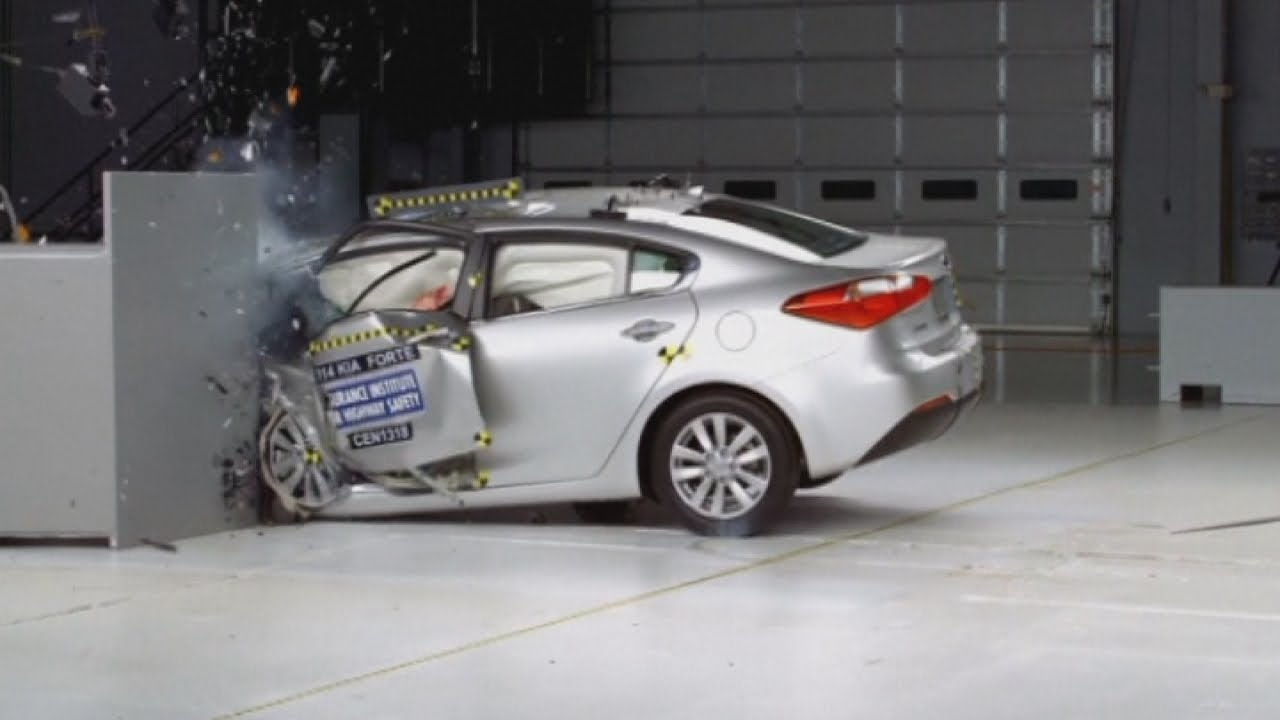
\includegraphics[width=\textwidth]{\docroot/998_figures/carcrashtest.jpg}
  \caption*{Car passengers protection test}
\end{minipage}}
}
\end{wrapfigure}
Testing is different from trying. Testing is war. In mechanical
engineering a strength test means abusing the material until it breaks. Same in the
modern card industry, where they run brand new cars into concrete walls
or into each other, to see how that car deals with unwanted circumstances.
They test by intending to break it, to ensure that the failure is
sufficiently graceful to cause no harm to passenger or innocent bystander.

Of course, ``normal'' usage is also tested, to ensure that the user
experience is what may be expected of the intended quality level. In
the car industry it can go as far as testing the sound of the doors closing.

%keep away from  wrap
%\vspace{4\baselineskip}
So should software testers. 
%\begin{multicols}{2}
\begin{itemize*}
\item Ensure that the software is fit for its
purpose,
\item but also survives un-purposeful (ab)use.
\end{itemize*}
%\end{multicols}
In the later case, in particular the survival, safety and security of the environment is
paramount. All to often a weak spot or vulnerability in an
application or library exposes risk to the operating system, files or
file systems of the system the application runs on. Example are
numerous. It might come unexpected, but a picture (e.g. a jpeg file)
can be forged to make an application crash or worse, execute alien, malicious code.
\section{Analyse and Design Top Down, Assemble Bottom Up}
todo

\subsection{Allow Maximise Ignorance}
One of the important design rule in good software design is \textit{proper
encapsulation}, meaning that you hide the implementation for the
user\footnote{The programmer using a class etc.}, assuming that she
honours the pre- and post conditions, by reading and understanding the
public \textit{documentation}, which can be used as the interface
provided to said user.

This puts the plight to ensure proper working of the component in all
circumstances on the implementer of the component. Too often 

\end{document}
